\documentclass[11pt]{article}
\usepackage[utf8]{inputenc}	% Para caracteres en español
\usepackage{amsmath,amsthm,amsfonts,amssymb,amscd}
\usepackage{multirow,booktabs}
\usepackage[table]{xcolor}
\usepackage{fullpage}
\usepackage{graphicx}
\usepackage{lastpage}
\usepackage{enumitem}
\usepackage{fancyhdr}
\usepackage{mathrsfs}
\usepackage{wrapfig}
\usepackage{setspace}
\usepackage{calc}
\usepackage{multicol}
\usepackage{cancel}
\usepackage[margin=3cm]{geometry}
\usepackage{amsmath}
\newlength{\tabcont}
\setlength{\parindent}{0.0in}
\setlength{\parskip}{0.05in}
\usepackage{empheq}
\usepackage{framed}
\usepackage{xcolor}
\colorlet{shadecolor}{orange!15}
\parindent 0in
\parskip 12pt
\geometry{margin=1in, headsep=0.25in}
\theoremstyle{definition}
\newtheorem{defn}{Definition}
\newtheorem{reg}{Rule}
\newtheorem{exer}{Exercise}
\newtheorem{note}{Note}
\begin{document}
\setcounter{section}{0}
\title{Review Notes}

\thispagestyle{empty}

\begin{center}
{\LARGE \bf Summer Intern Lectures}\\
{\large Time Series Analysis Team}\\
June 2017
\end{center}
\section{Principal Component Analysis (PCA)}
\subsection{Why use it?}
We are lucky to have lots of data available to us, data that has information and that we want to use for analysis and prediction. 101 econometric tools, however, have a limitation in this respect: overfitting. Regressing a dependent variable over a large set of predictors will make the estimation fit to the idiosyncracies (the $\varepsilon$) of the data given good in-sample results but bad out-of-sample results.

\begin{shaded}
\textbf{Example 1} \newline
Below we regress Non-farm Payrolls (in change from the previous period) over 33 other monthly macroeconomic series. The estimation is performed from the end of 2009 to the beginning of 2015. The fit (the red line) is quite close to the actual data series in this period. Once we bring forward the fit out-of-sample (with the same estimation from 2015, the series performs very poorly (the green line is not a good fit to the blue line after 2015).
%\begin{figure}
\begin{center}
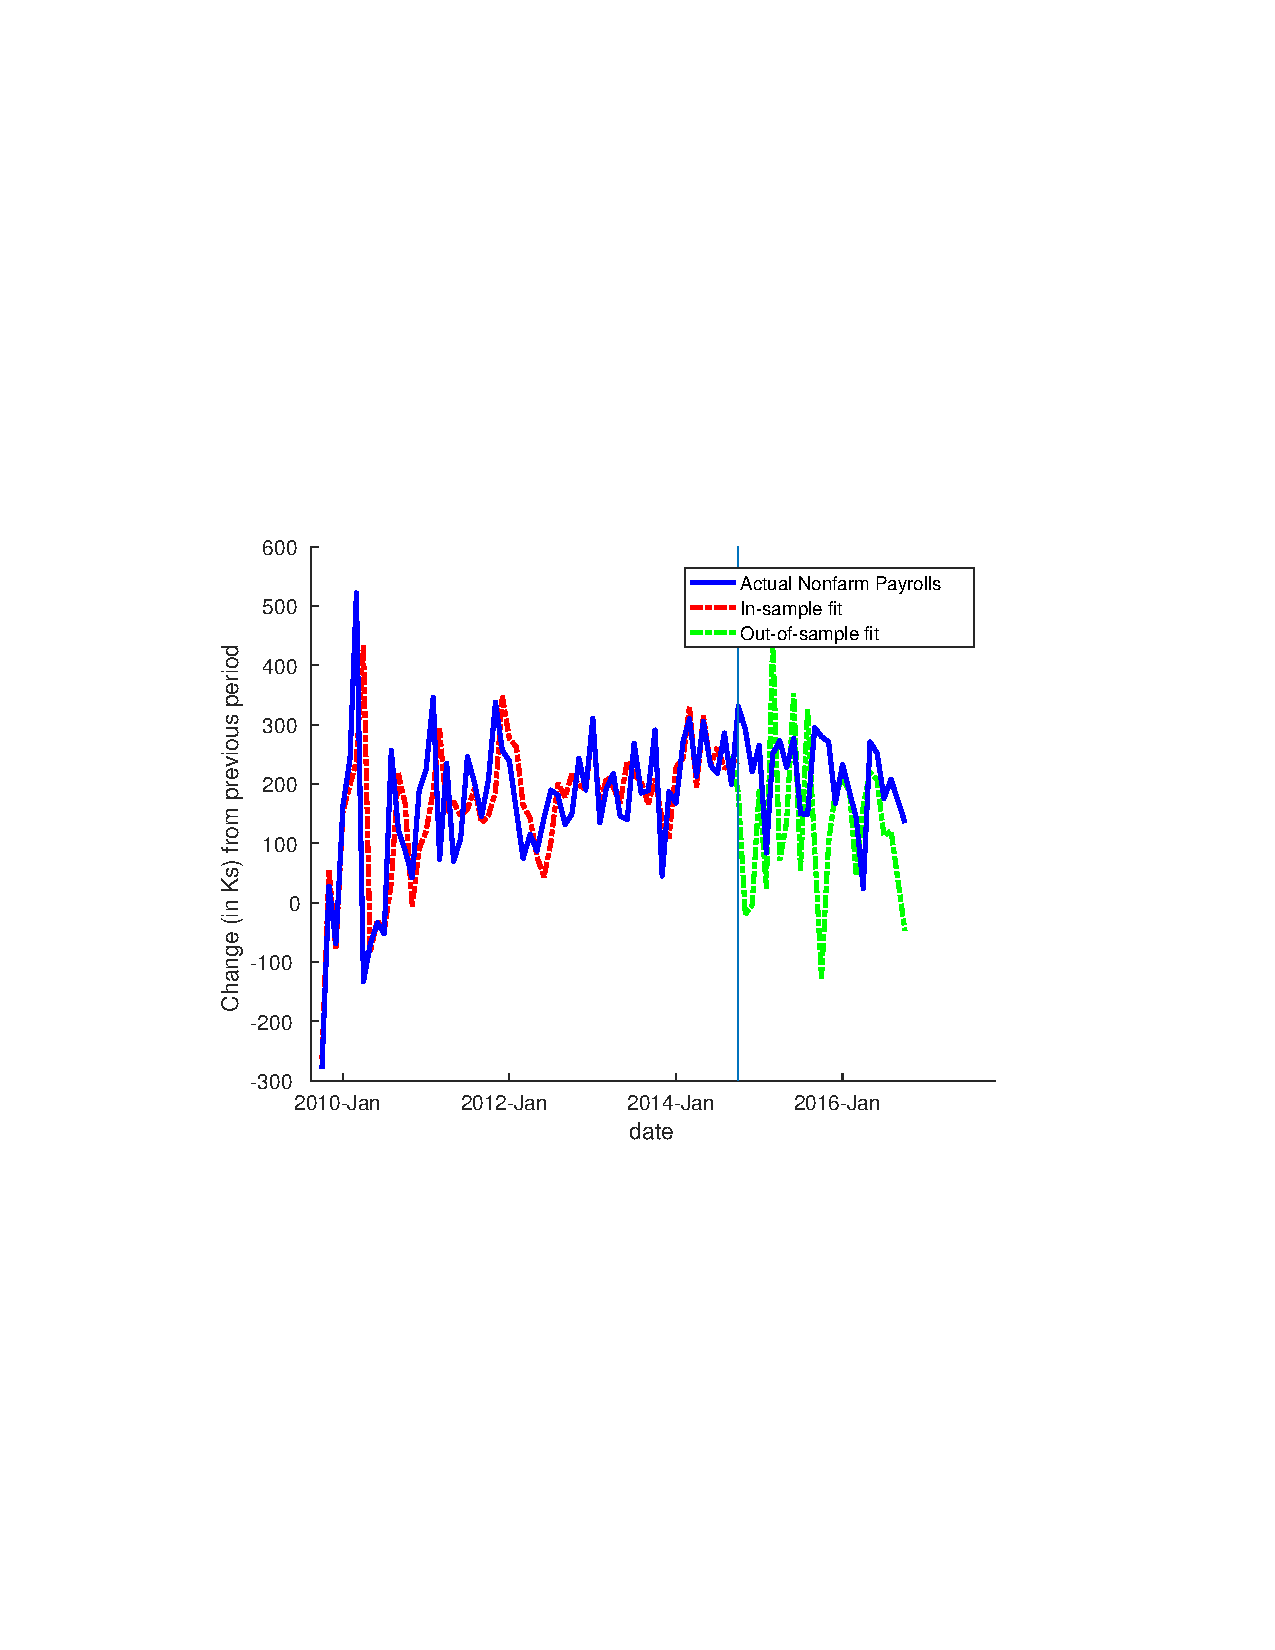
\includegraphics[scale=0.6,trim={0cm, 8cm, 0cm, 8cm}, clip]{plots/cursefit.pdf}
\end{center}
%\end{figure}
\end{shaded}			

We like the variation that lots of data gives us but we do not want to overfit. How to deal with this problem? One way is to use principal component analysis which allows to extract a lot of the data's variation while reducing the dimensionality of the problem and thus preventing overfitting.

\subsection{Methodology}
We have a data set $X$ of dimension $T\times n$ where $T$ is the number of observations for each series and $n$ is the number of series considered.
\begin{itemize}
\item[step 1:] \textbf{Normalize the data}\newline
One aim of PCA is to capture lots of the variance in the data. However, if data series are not ``comparable'', series that have a larger magnitude will be given higher weight given that their variance will naturally be higher. For example, Nonfarm Payrolls (measured in level change from previous period) in the data set contained in this folder, has standard deviation of $\approx 200$ while the standard deviation of unemplont (also measured in level change from previous period) is around $0.6$. This is obvious since nonfarm payrolls is measured in thousands and the unemployment rate is measured in percentage points. 

Given the data $X$, do the following

\begin{equation}
{\tilde{X}}_{:,i} = \frac{X_{:,i}-\mu(X_{:,i})}{\sigma(X_{:,i})}
\end{equation}

where $\mu(X,1)$ and $\sigma(X,1)$ are the means and standard deviations of each column of X, i.e. of each data series in X. $\tilde{X}$ will be our normalized data set.

\item[step 2:] \textbf{Compute covariance matrix and its eigenvectors and eigenvalues}\newline
What PCA aims to get is the direciton(s) along wich the data move the most. The covariance matrix of the data ($\Omega$) contains an information about this variation. $\Omega$ will be a $n\times n$ matrix symmetric around the main diagonal. The eigenvectors of $\Omega$ will be, if they exist, $n$ and will be orthogonal to each other indicating the direction in which the data varies according to the magnitude of their corresponding eigenvalue (the higher the eigenvalue, the more the data varies along the direction of that eigenvector). We will denote the eigenvector matrix by $Evec = [\vec{e}_{1}\cdots \vec{e}_{n}]$ and the eigenvalue matrix as $Eval = [e_{1} \cdots e_{n}]$. PCA will enable us to write the data as linear combination of the eigenvectors.
\begin{shaded}
\textbf{Example 2} \newline
Lets look at a two-dimensional data set. Here we show standardized payrolls and JOLTS plotted against each other as well as the eigenvectors of their variance-covariance matrix.
\begin{center}
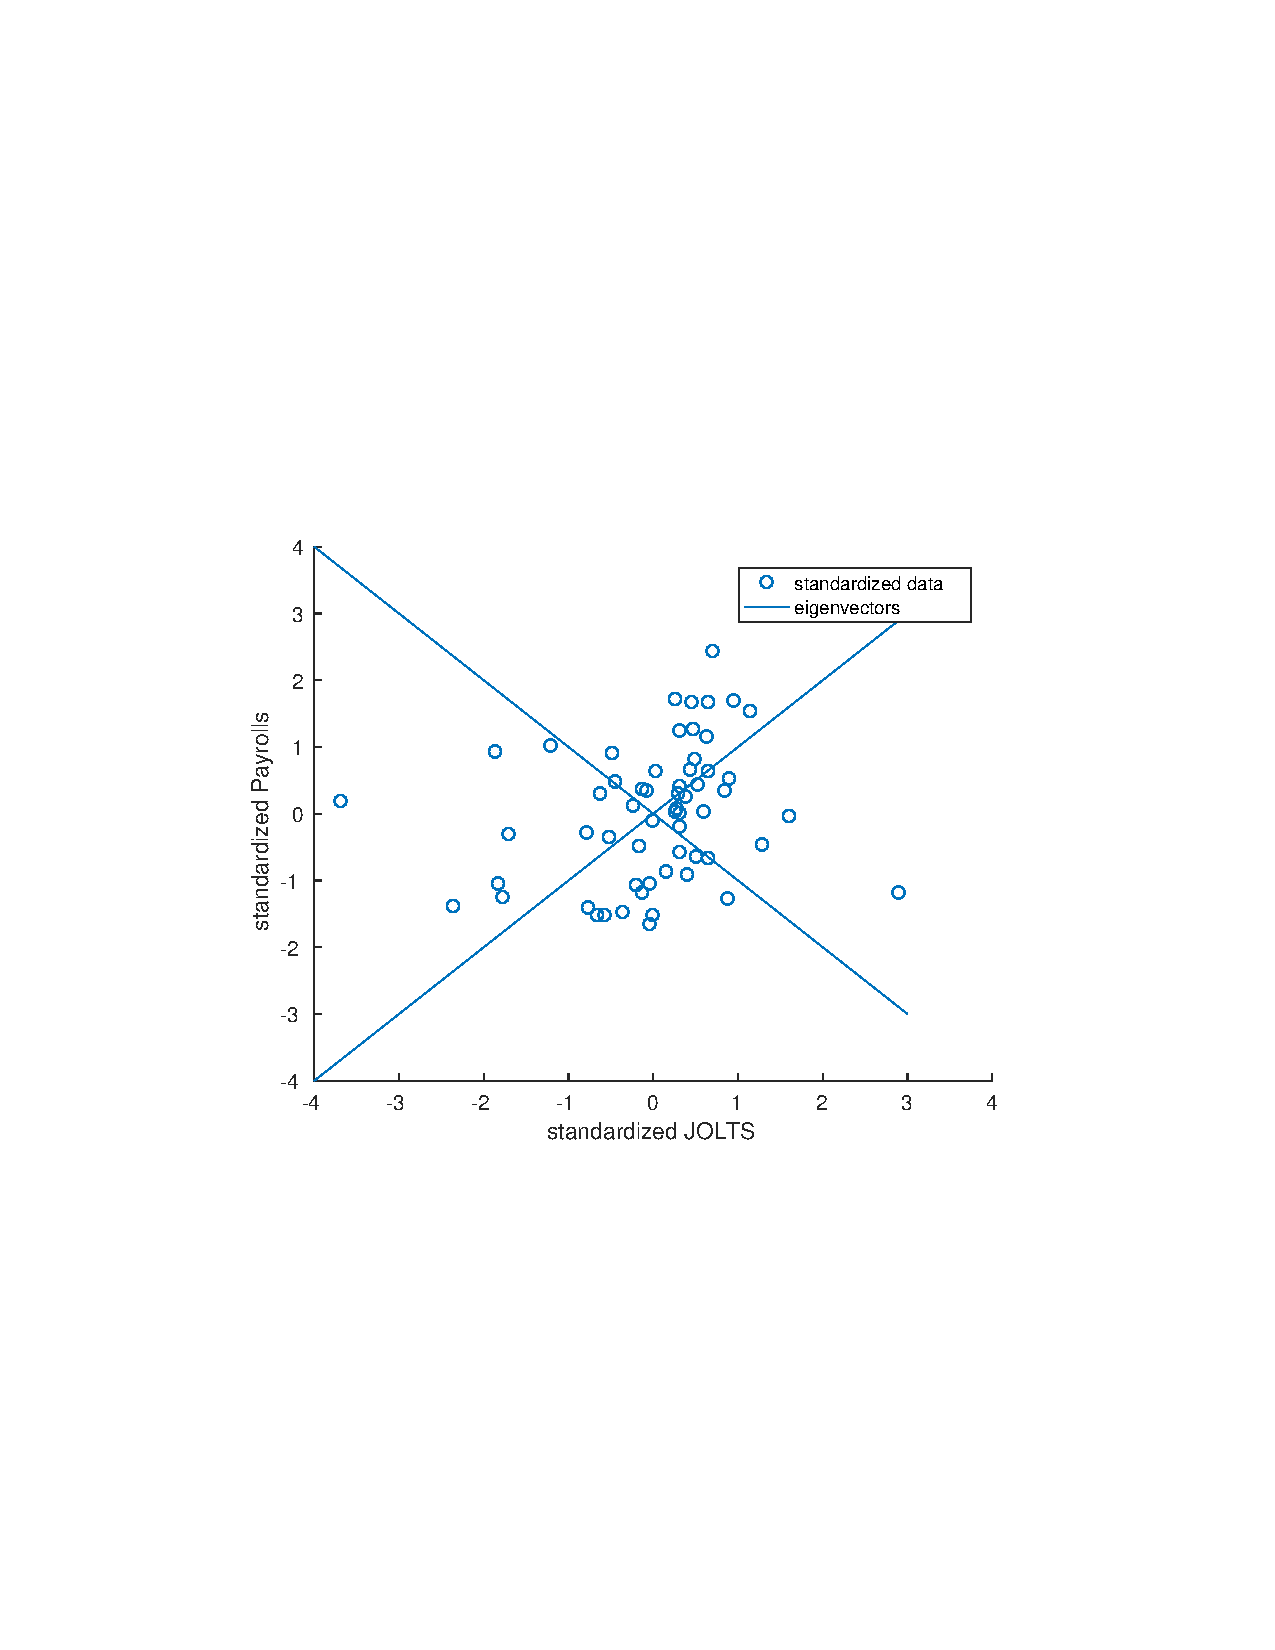
\includegraphics[scale=0.45,trim={0cm, 8cm, 0cm, 8cm}, clip]{plots/eig_plot.pdf}
\end{center}
\end{shaded}			

\item[step 3:]\textbf{Reducing dimensionality}\newline
Here comes the second beauty of PCA. Since the first few eigenvectors will register most of the variation of the data (in general, certianly true with macroeconomic variables), one can study the data ``projected'' on these few eigenvectors reducing considerably the dimensionality of the data set which allows us to overcome the curse of dimensionality problem. So the next step will be deciding how many eigenvectors to consider, suppose you take $p\leq n$ (note, if $p=n$ then our data will be unchanged, projected onto itself). We then fom the feature vectors of chosen eigenvectors, this is also known as the loadings vector indicating how each series loads on each principal component: 
\begin{equation}FV = [\vec{e}_{1} \cdots \vec{e}_{p}].
\end{equation}

Finally, to get the principal compoents, we simply put the loadings and the transformed raw data together:

\begin{equation}
PCA = FV'\cdot \tilde{X}'
\end{equation}

\begin{shaded}
\textbf{Example 3: Predicting with PCA} \newline
Often principal components are used as dependent variables in regressions. They contain a lot of information yet are few and do not cause overfitting so they are great candidates as right-hand-side variables. Here we regress (standardized) nonfarm payrolls over the first four principal components of the standardized data set.
$$\tilde{NFP} = \alpha + \vec{\beta}'\cdot PCA + \epsilon.$$ 
Note that $\alpha \approx 0$ and will unlikely be significant since we have demeaned the data. We can then get the out-of-sample forecast for the variable after we un-standardize it as follows:
$$NFP_{forecast} = \tilde{NFP}*std(NFP)+mean(NFP).$$
Notice that the forecast has improved considerably because we were able to store the useful information from the rich data set without fitting to the errors.
\begin{center}
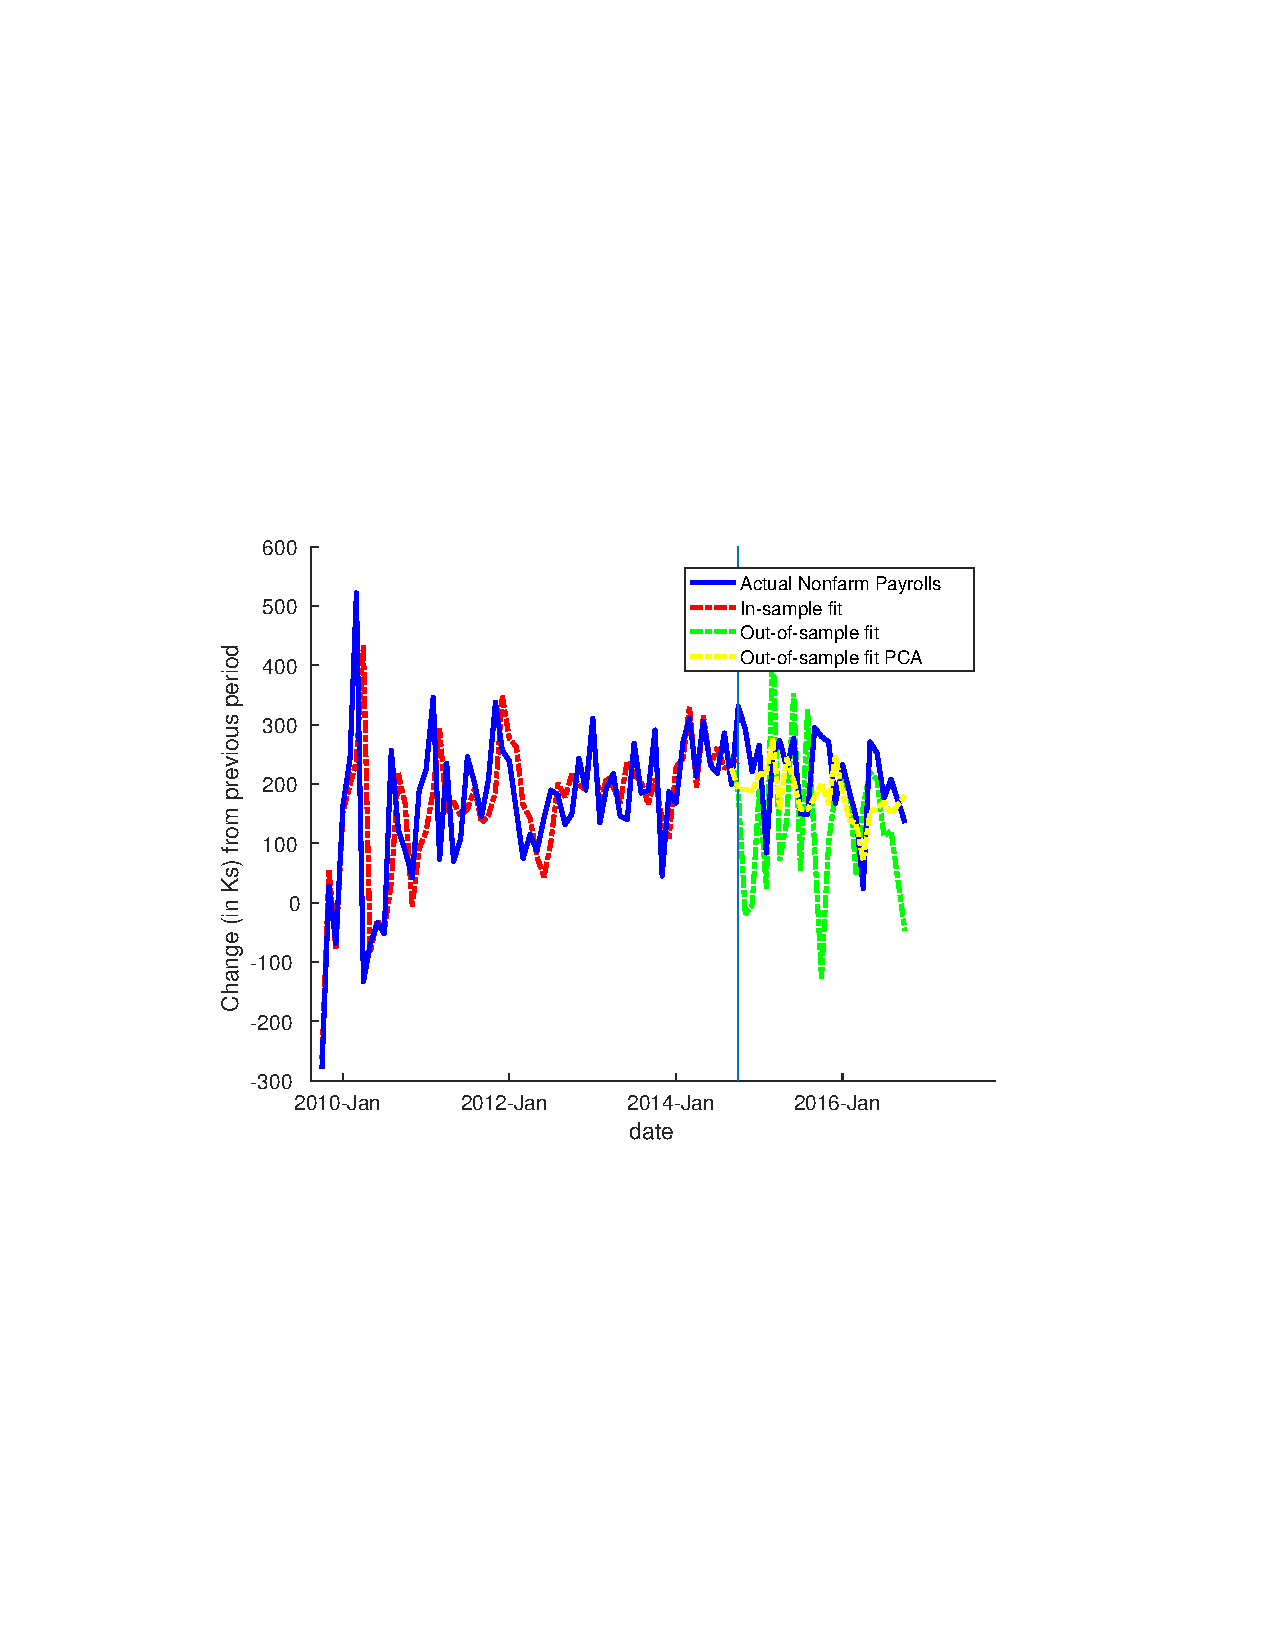
\includegraphics[scale=0.6,trim={0cm, 8cm, 0cm, 8cm}, clip]{plots/cursefitPCA.pdf}
\end{center}
\end{shaded}			


\end{itemize}

\end{document}